\documentclass[runningheads, envcountsame, a4paper]{llncs}
\usepackage[T1]{fontenc}
\usepackage{color}
\usepackage{amsmath, amssymb}
\usepackage{tikz}
\usetikzlibrary{shapes,calc,math,backgrounds,matrix}

\begin{document}

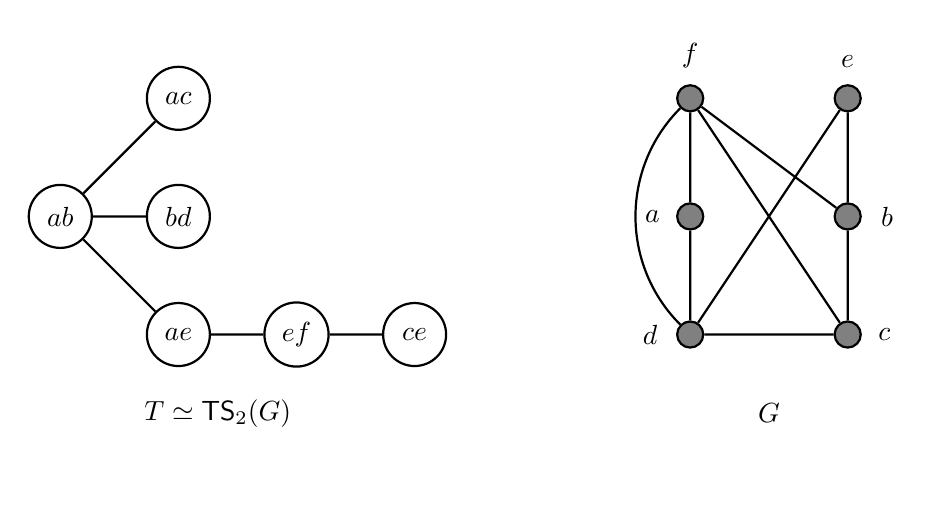
\begin{tikzpicture}[every node/.style={circle, draw, thick, minimum size=0.8cm}]
\begin{scope}
\node (v1) at (0,0) {$ab$};
\node (v2) at (1.5,1.5) {$ac$};
\node (v3) at (1.5,0) {$bd$};
\node (v4) at (1.5,-1.5) {$ae$};
\node (v5) at (3,-1.5) {$ef$};
\node (v6) at (4.5,-1.5) {$ce$};

\draw[thick] (v1) -- (v2) (v1) -- (v3) (v1) -- (v4) -- (v5) -- (v6);

\node[draw=none] (T) at (2,-2.5) {$T \simeq \mathsf{TS}_2(G)$};
\end{scope}
\begin{scope}[shift={(8,0)}, every node/.style={circle, draw, thick, fill=gray, minimum size=0.3cm}]
\node[label=left:$a$] (a) at (0,0) {};
\node[label=right:$b$] (b) at (2,0) {};
\node[label=right:$c$] (c) at (2,-1.5) {};
\node[label=left:$d$] (d) at (0,-1.5) {};
\node[label=above:$e$] (e) at (2,1.5) {};
\node[label=above:$f$] (f) at (0,1.5) {};

\draw[thick] (b) -- (c) (a) -- (d) (d) -- (c) (e) -- (b) (e) -- (d) (a) -- (f) (b) -- (f) (c) -- (f) (d) edge[bend left=45] (f);

\node[draw=none, fill=none] (G) at (1,-2.5) {$G$};
\end{scope}
\end{tikzpicture}

\end{document}